\documentclass[12pt,letterpaper]{article}

\usepackage[T1]{fontenc}
\usepackage[utf8]{inputenc}
\usepackage[spanish,mexico,es-tabla,es-noshorthands]{babel}
\usepackage{newtxtext,newtxmath}          % Times New Roman
\usepackage[margin=2.5cm]{geometry}
\usepackage{graphicx}
\usepackage{float}
\usepackage{caption}
\usepackage{subcaption}
\usepackage{booktabs}
\usepackage{enumitem}
\usepackage{amsmath}          % no cargar amssymb: choca con \Bbbk de newtxmath
\usepackage{listings}
\usepackage{xcolor}
\usepackage{setspace}
\usepackage[colorlinks=true,allcolors=black]{hyperref}
\usepackage{todonotes}                    % usar [disable] para la versión final

\graphicspath{{evidencias/}{../assets/}}
\captionsetup{labelsep=colon,font=small,labelfont=bf}
\onehalfspacing
\setlength{\parskip}{6pt}

% Títulos de sección al estilo del formato de la profesora
\usepackage{titlesec}
\titleformat{\section}{\normalfont\large\bfseries}{}{0pt}{}
\titleformat{\subsection}{\normalfont\normalsize\bfseries}{}{0pt}{}

\definecolor{codekw}{RGB}{0,0,180}
\definecolor{codecm}{RGB}{0,128,0}
\definecolor{codestr}{RGB}{170,0,0}
\definecolor{codebg}{RGB}{248,248,248}

\lstdefinestyle{hdl}{
  language=VHDL,
  basicstyle=\ttfamily\footnotesize,
  keywordstyle=\color{codekw}\bfseries,
  commentstyle=\color{codecm}\itshape,
  stringstyle=\color{codestr},
  backgroundcolor=\color{codebg},
  numbers=left, numberstyle=\tiny\color{gray}, numbersep=8pt,
  frame=single, rulecolor=\color{gray!50},
  breaklines=true, breakatwhitespace=true,
  tabsize=2, showstringspaces=false, captionpos=b,
  extendedchars=true, inputencoding=utf8,
  literate={á}{{\'a}}1 {é}{{\'e}}1 {í}{{\'i}}1 {ó}{{\'o}}1 {ú}{{\'u}}1
           {Á}{{\'A}}1 {É}{{\'E}}1 {Í}{{\'I}}1 {Ó}{{\'O}}1 {Ú}{{\'U}}1
           {ñ}{{\~n}}1 {Ñ}{{\~N}}1 {ü}{{\"u}}1 {¿}{{?`}}1 {¡}{{!`}}1
}
\lstset{style=hdl}
\renewcommand{\lstlistingname}{Figura}   % el código se numera junto a las figuras


\begin{document}

\begin{titlepage}
\centering
\noindent
\begin{minipage}[c]{0.45\textwidth}\centering
  
\includegraphics[height=3.2cm]{logo-unam.jpg}
\end{minipage}\hfill
\begin{minipage}[c]{0.45\textwidth}\centering
  
\includegraphics[height=3.2cm]{logo-fi.png}
\end{minipage}

\vspace{1.2cm}
{\Large\bfseries UNIVERSIDAD NACIONAL AUTÓNOMA\\[2pt] DE MÉXICO\par}
\vspace{0.9cm}
{\large\bfseries FACULTAD DE INGENIERÍA\par}
\vspace{0.6cm}
{\large\bfseries INGENIERÍA EN COMPUTACIÓN\par}
\vspace{0.6cm}
{\bfseries Laboratorio de Organización de Arquitectura de Computadoras\par}
\vspace{0.9cm}
{\bfseries Reporte - Introducción a las herramientas de desarrollo de los FPGAs\par}

\vspace{1.6cm}
\raggedright
{\bfseries NOMBRE DE LOS INTEGRANTES:}\\
Omar Alfonso Zendejas Labias \quad Grupo de Teoría: 04

\vspace{1.8cm}
{\bfseries NOMBRE DEL PROFESOR: ING. KAREN PÉREZ}

\vspace{0.6cm}
{\bfseries GRUPO: 06}

\vspace{0.6cm}
{\bfseries SEMESTRE:} \underline{2027-1.}

\vspace{0.6cm}
\hfill {\bfseries FECHA DE ENTREGA: 3 de septiembre de 2026}
\thispagestyle{empty}
\end{titlepage}

\setcounter{page}{1}

\section{Objetivo}

En esta práctica se buscó que el alumno se familiarizara con el entorno de desarrollo
Quartus Prime Lite Edition y con el flujo básico de diseño de sistemas digitales sobre
una tarjeta de desarrollo basada en \textit{FPGA}. A partir de la creación y
configuración de un proyecto, la captura de un diagrama esquemático, su compilación, la
asignación de señales de entrada y salida, y la realización de una simulación funcional
mediante el \textit{Simulation Waveform Editor}, se buscó que el alumno adquiriera la
capacidad de llevar un diseño digital desde su concepción hasta su programación en una
tarjeta FPGA.

\section{Introducción}

Un \textit{Field Programmable Gate Array} (FPGA) es un dispositivo digital
reconfigurable compuesto por una matriz de bloques lógicos y recursos de interconexión
programables, que permiten implementar prácticamente cualquier circuito digital
combinacional o secuencial sin necesidad de fabricar un circuito integrado dedicado.
Para diseñar sobre estos dispositivos se emplean herramientas de diseño asistido por
computadora (\textit{Computer-Aided Design}, CAD); en el caso de los dispositivos de la
familia MAX 10 utilizados en este laboratorio, la herramienta correspondiente es Quartus
Prime, en su edición Lite.

Quartus Prime permite capturar un diseño de dos formas principales: mediante lenguajes
de descripción de hardware (como VHDL o Verilog) o mediante \textit{schematic entry},
es decir, dibujando directamente el circuito con símbolos de compuertas lógicas
interconectadas. Esta segunda modalidad es la que se utilizó en la presente práctica, en
la cual el circuito se construyó a partir de compuertas XOR, NAND, OR, NOR y AND, cuyo
comportamiento se rige por las reglas del álgebra booleana descritas, entre otros, por
Mano y Ciletti \cite{mano}. Una vez capturado y compilado el diseño, su comportamiento
lógico puede verificarse antes de programarlo físicamente mediante una simulación
funcional, en la que se generan formas de onda para las entradas y se observa la
respuesta calculada para las salidas a través del \textit{Simulation Waveform Editor}.

\section{Desarrollo}

\subsection{Creación del proyecto}

Se creó un nuevo proyecto en Quartus Prime Lite Edition mediante el asistente
\textit{New Project Wizard}, seleccionando como familia de dispositivo MAX 10
(DA/DF/DC/SA/SC), tal como lo indica el manual de la práctica. Dado que para esta
sesión no se contó con la tarjeta de desarrollo física, se conservó el dispositivo
asignado por defecto dentro de dicha familia en lugar de seleccionar manualmente un
modelo específico. Como herramienta de simulación se configuró ModelSim-Altera con
formato VHDL, de acuerdo con lo especificado en el manual.

\subsection{Diseño esquemático}

Una vez creado el proyecto, se agregó un archivo de tipo \textit{Block Diagram/Schematic
File} y se construyó el circuito combinacional solicitado, con tres entradas (A, B y C)
y una salida (S), utilizando compuertas XOR, NAND, OR, NOR y AND interconectadas según
se muestra en la figura \ref{fig:diagrama}.

\begin{figure}[H]
  \centering
  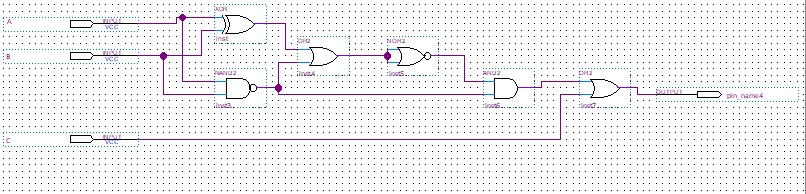
\includegraphics[width=0.8\textwidth]{01-diagrama-only.jpeg}
  \caption{Diagrama esquemático del circuito combinacional implementado en Quartus
    Prime, con entradas A, B, C y salida S.}
  \label{fig:diagrama}
\end{figure}

Las entradas A y B alimentan una compuerta XOR y una compuerta NAND. Las salidas de
estas dos compuertas se combinan mediante una compuerta OR y, posteriormente, mediante
una compuerta NOR, para finalmente combinarse de nuevo con la salida de la compuerta
NAND en una compuerta AND. El resultado de esta red de cinco compuertas se combina, por
último, con la entrada C mediante la compuerta OR final (renombrada con el apellido del
alumno, conforme lo pide el manual) para producir la salida S.

Analizando la red mediante álgebra booleana puede verificarse que, para las entradas A
y B, la salida de la compuerta OR (que combina el XOR y el NAND de A y B) es
equivalente al propio NAND de A y B, ya que el XOR nunca vale 1 cuando el NAND vale 0.
La compuerta NOR posterior invierte ese resultado, entregando el AND de A y B; y la
compuerta AND final de esta subred combina dicho valor con el NAND de A y B, que es su
complemento, por lo que el resultado es siempre 0 independientemente de A y B:

\begin{align}
  \text{or}_1 &= (A \oplus B) + \overline{AB} = \overline{AB} \label{eq:or1}\\
  \text{nor}_1 &= \overline{\text{or}_1 + \overline{AB}} = AB \label{eq:nor1}\\
  \text{and}_1 &= \text{nor}_1 \cdot \overline{AB} = AB \cdot \overline{AB} = 0
    \label{eq:and1}
\end{align}

Como la compuerta OR final combina este valor constante (ecuación \ref{eq:and1}) con la
entrada C, la salida del circuito se reduce a $S = 0 + C = C$ para cualquier
combinación de A y B. Esta reducción algebraica es consistente con el comportamiento
observado durante la simulación funcional, descrita en la sección siguiente.

\subsection{Simulación funcional}

Para verificar el comportamiento del circuito se creó un archivo de tipo
\textit{University Program VWF} mediante el \textit{Simulation Waveform Editor}. Las
señales A, B, C y S se insertaron utilizando la herramienta \textit{Node Finder},
copiando todos los nodos encontrados a la lista de nodos seleccionados. Posteriormente
se generaron, sobre las entradas A, B y C, las ocho combinaciones posibles
(000, 001, 010, 011, 100, 101, 110 y 111) solicitadas en el manual, y se ejecutó la
simulación funcional (\textit{Run Functional Simulation}).

\subsubsection{Tabla de verdad}

A partir del comportamiento observado en la simulación, la tabla de verdad del circuito
es la siguiente:

\begin{table}[H]
  \centering
  \begin{tabular}{ccc|c}
    \toprule
    A & B & C & S \\
    \midrule
    0 & 0 & 0 & 0 \\
    0 & 0 & 1 & 1 \\
    0 & 1 & 0 & 0 \\
    0 & 1 & 1 & 1 \\
    1 & 0 & 0 & 0 \\
    1 & 0 & 1 & 1 \\
    1 & 1 & 0 & 0 \\
    1 & 1 & 1 & 1 \\
    \bottomrule
  \end{tabular}
  \caption{Tabla de verdad del circuito combinacional.}
  \label{tab:verdad}
\end{table}

Como se aprecia en la tabla \ref{tab:verdad}, la salida S coincide en todos los casos
con el valor de la entrada C, sin depender de A ni de B, lo cual concuerda con la
reducción algebraica presentada en la ecuación \ref{eq:and1}.

\section{Análisis de resultados}

Durante la primera ejecución de la simulación se obtuvo el resultado mostrado en la
figura \ref{fig:error}, en el cual la salida S permanece en estado desconocido (X)
durante toda la simulación, a pesar de que las entradas A, B y C sí presentan las
transiciones configuradas.

\begin{figure}[H]
  \centering
  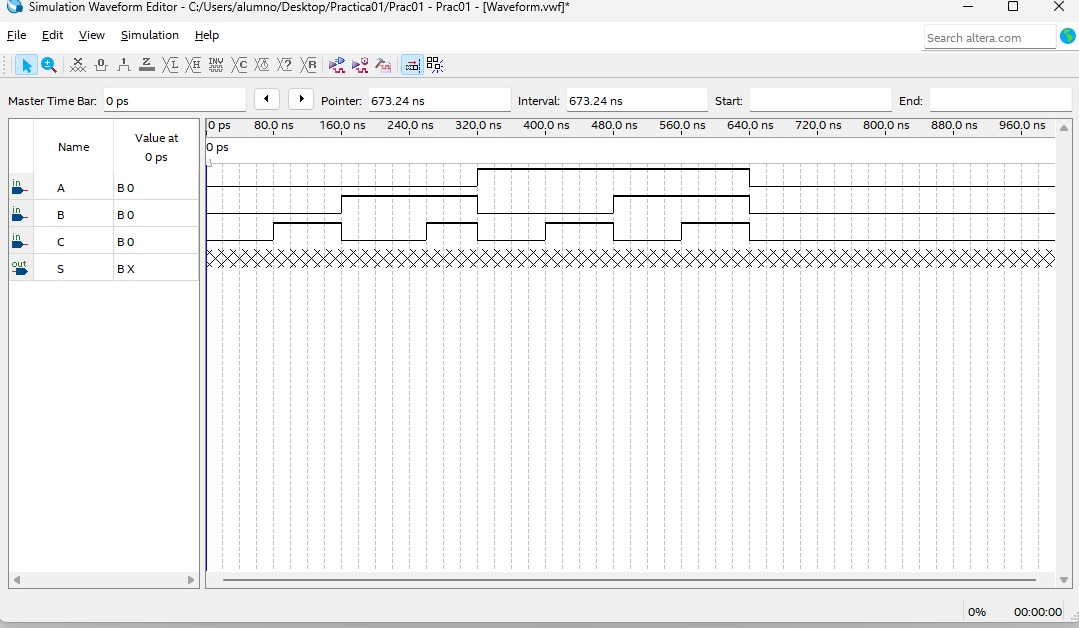
\includegraphics[width=0.8\textwidth]{02-resultado-error.jpeg}
  \caption{Simulación funcional con salida en estado desconocido (X), evidencia de una
    conexión incorrecta en el diseño.}
  \label{fig:error}
\end{figure}

Este resultado corresponde al fallo lógico ante el cual advierte el manual de la
práctica. En este caso el problema no estuvo en el cableado del esquemático, sino en la
ubicación del proyecto: éste se había creado directamente en la raíz del equipo, lo que
generaba conflictos y no dejaba que la simulación resolviera un valor lógico definido
para S. La corrección consistió en cerrar Quartus Prime por completo y volver a crear el
proyecto, con el mismo diagrama, dentro de una carpeta dedicada en lugar de la raíz.

Tras rehacer el proyecto de esta manera, se volvió a ejecutar la simulación funcional,
obteniéndose el resultado mostrado en la figura \ref{fig:correcto}.

\begin{figure}[H]
  \centering
  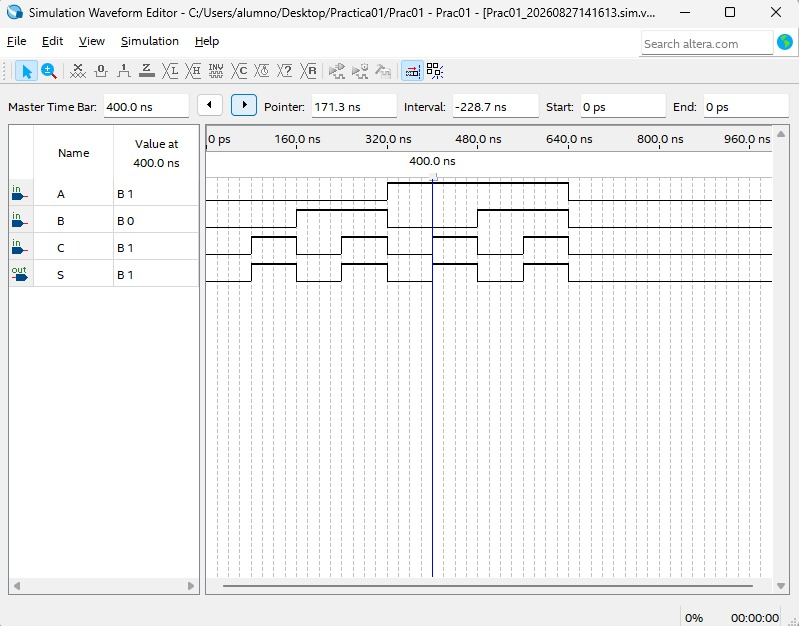
\includegraphics[width=0.8\textwidth]{02-resultado.jpeg}
  \caption{Simulación funcional correcta mostrando las ocho combinaciones de entrada y
    el valor resultante de la salida S.}
  \label{fig:correcto}
\end{figure}

En este segundo resultado, la salida S sí toma valores lógicos definidos y, para cada
una de las ocho combinaciones de entrada generadas, reproduce el valor de la entrada C,
tal como se anticipó en la tabla \ref{tab:verdad}. Por ejemplo, en el instante marcado
por la barra de tiempo (400.0 ns), con A = 1, B = 0 y C = 1, la salida observada es
S = 1, consistente con S = C.

La etapa de asignación de pines y programación de la tarjeta FPGA no se abordó en esta
sesión, ya que aún no se trabajó con la tarjeta física; dicha etapa se cubrirá en una
práctica posterior.

\section{Conclusiones individuales}

\subsection{Omar Alfonso Zendejas Labias}

El objetivo de la práctica se cumplió: logré crear el proyecto en Quartus Prime, capturar
el diagrama esquemático con las compuertas indicadas y simular su funcionamiento con el
Simulation Waveform Editor. El único inconveniente fue que la primera simulación
arrojaba la salida S en estado desconocido (X); esto no se debía al circuito, sino a que
el proyecto se había creado en la raíz del equipo, así que lo rehice dentro de una
carpeta y con eso la simulación arrojó valores definidos. Como resultado, la tabla de
verdad confirma que la salida S siempre es igual a la entrada C, sin depender de A ni de
B. Queda pendiente la etapa de asignación de pines y programación en la tarjeta física,
que aún no se ha trabajado en el curso.

\begin{thebibliography}{9}
\bibitem{mano} M. M. Mano y M. D. Ciletti, \emph{Diseño digital}, 5a ed.
  Naucalpan de Juárez, México: Pearson Educación, 2013.
\end{thebibliography}

\end{document}
